\documentclass[11pt,a4paper,oneside]{article}
\usepackage[danish]{babel}	
\usepackage[utf8]{inputenc}
\usepackage{listings}
\usepackage{graphicx}
\usepackage{float}
\usepackage[margin=1in]{geometry}
\usepackage{fancyhdr}
\pagestyle{fancy}
\usepackage{color}
\usepackage{tabu}
\usepackage{multirow}
\usepackage{baskervald}
\usepackage[T1]{fontenc}
\setlength{\parindent}{0mm}
\setlength{\parskip}{5mm}    
\usepackage{tabularx}
\usepackage{amsmath}
\usepackage[hidelinks]{hyperref}


\renewcommand{\figureautorefname}{Figur}
\renewcommand{\headrulewidth}{0pt}
\renewcommand{\footrulewidth}{0pt}
\headheight = 25pt

%\setcounter{tocdepth}{1} % Show sections
\setcounter{tocdepth}{2} % + subsections
%\setcounter{tocdepth}{3} % + subsubsections
%\setcounter{tocdepth}{4} % + paragraphs
%\setcounter{tocdepth}{5} % + subparagraphs


%MATHLAB
\usepackage{color} %red, green, blue, yellow, cyan, magenta, black, white
\definecolor{mygreen}{RGB}{28,172,0} % color values Red, Green, Blue
\definecolor{mylilas}{RGB}{170,55,241}

\lstset{language=Matlab,%
	%basicstyle=\color{red},
	breaklines=true,%
	morekeywords={matlab2tikz},
	keywordstyle=\color{blue},%
	morekeywords=[2]{1}, keywordstyle=[2]{\color{black}},
	identifierstyle=\color{black},%
	stringstyle=\color{mylilas},
	commentstyle=\color{mygreen},%
	showstringspaces=false,%without this there will be a symbol in the places where there is a space
	numbers=left,%
	numberstyle={\tiny \color{black}},% size of the numbers
	numbersep=9pt, % this defines how far the numbers are from the text
	emph=[1]{for,end,break},emphstyle=[1]\color{red}, %some words to emphasise
	%emph=[2]{word1,word2}, emphstyle=[2]{style},    
}




\begin{document}
	\begin{titlepage}
	
	
	
	\newcommand{\HRule}{\rule{\linewidth}{0.5mm}} % Defines a new command for the horizontal lines, change thickness here
	\setlength{\topmargin}{0in}
	\centering % Center everything on the page
	
	%----------------------------------------------------------------------------------------
	%	HEADING SECTIONS
	%----------------------------------------------------------------------------------------
	\textsc{\LARGE Aarhus universitet}\\[1.5cm] % Name of your university/college
	\textsc{\Large Adaptive Control and Automation}\\[0.5cm] % Major heading such as course name
	\textsc{\large 7. Semester}\\[0.5cm] % Minor heading such as course title
	
	%----------------------------------------------------------------------------------------
	%	TITLE SECTION
	%----------------------------------------------------------------------------------------
	
	\HRule \\[0.4cm]
	{ \huge \bfseries ACA projekt}\\ % Title of your document
	\HRule \\[1cm]
	
	%----------------------------------------------------------------------------------------
	%	AUTHOR SECTION
	%----------------------------------------------------------------------------------------
	
	\begin{minipage}{0.4\textwidth}
		\begin{flushleft} \large
			\emph{Gruppemedlemmer:}\\
			Søren Landgrebe \\
			Tim Hede Stenholt Jensen \\
		\end{flushleft}
	\end{minipage}
	~
	\begin{minipage}{0.4\textwidth}
		\begin{flushright} \large
			\emph{Studienr:} \\
			201508295\\
			201508449\
		\end{flushright}
	\end{minipage}\\[5cm]
	
	%----------------------------------------------------------------------------------------
	%	LOGO SECTION
	%----------------------------------------------------------------------------------------
	
	
\includegraphics[scale=0.5]{figur/logo.jpg}\\[1cm]
	
	%----------------------------------------------------------------------------------------
	%	DATE SECTION
	%----------------------------------------------------------------------------------------
	
	{\large \today}\\[0.5cm] % Date, change the \today to a set date if you want to be precise
	
	
	\vfill % Fill the rest of the page with whitespace
	
	\end{titlepage}


%TABLE OF CONTENTS
\tableofcontents

\pagebreak
\section{Introduktion}

Vores projekt tager udfordringen op med en mejetærsker (eller et andet køretøj), som har den problemstilling, at den kan komme ud i ujævnt terræn, hvormed at tanken på mejetærskeren kan få overbalance til den ene side og evt. tippe køretøjet eller tabe gods overbord. Ved at lave et system, som selv kan nivellere ”overkroppen” af køretøjet til vandret position, uanset ”underkroppens” vinkel, kan dette problem løses. Dette sikre at både kabinen og tanken på mejetærskeren altid vil være i vandret position vinkelret på køreretningen i ujævnt terræn.

\begin{figure}[H]
	\centering
	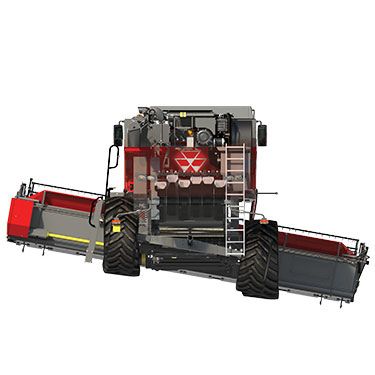
\includegraphics[width = 300pt]{figur/Visionbillede}
	\caption{Visionsbillede}
	\label{fig:konceptbillede}
\end{figure}

Kontrolsystemet kommer til at bestå med en motor, et gyroskop og en LEGO bil, hvor overdelen kan vippe sidelæns. Det forventes at systemet kan regulere en horisontal vinkel på op til ±30 grader tilbage til vandret i ”overdelen” ±1 grad. Systemet skal være adaptivt, idet mængden af gods/korn kan variere og dermed ændre belastningen på motoren.   \\ 



\pagebreak
\section{Krav til dynamikken}

I dette afsnit beskrives kravene til hvilken funktionalitet systemet har. Der er opstillet følgende række krav i første omgang.
\begin{itemize}
	\item Systemet kan regulere en horisontal vinkel på op til ±30 grader tilbage til vandret i ”overdelen”
	\item Overshoot max 5\%
	\item Settlingtime 0.5 sekund 
	\item Stationær fejl max 10\%  
	
\end{itemize}



Herunder i \autoref{fig:Blokdiagram} vises et blokdiagram, som viser en beskrivelse af systemets (fysiske) blokke, som beskriver opbygningen af systemet på Lego bilens styringsenhed. 


\begin{figure}[H]
	\centering
	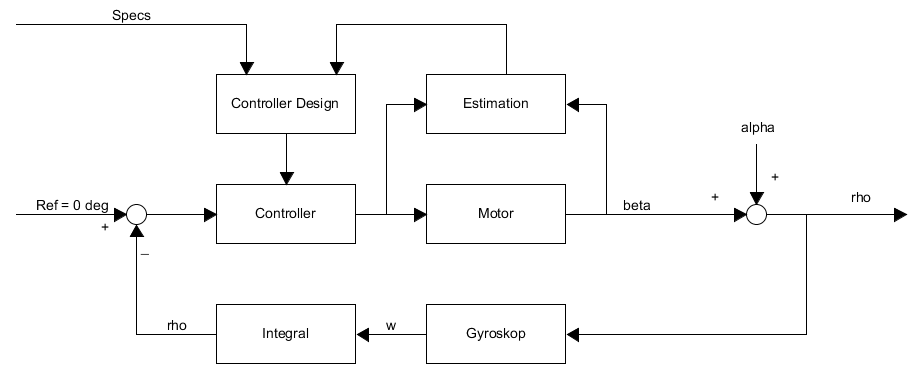
\includegraphics[width = 400 pt]{figur/blokdiagram.png}
	\caption{Blokdiagram}
	\label{fig:Blokdiagram}
\end{figure}

\textit{beta} er motorens vinkel,\textit{ alpha} er vinkel forstyrrelsen fra terrænets hældning. \textit{rho} er vinkelen på selve overdelen af Lego bilen. Det er denne vinkel \textit{rho}, som gerne forsøges at reguleres til 0 grader eller vandret. Outputtet fra gyroskopet er en vinkelhastighed som igennem integration laves om til en vinkel ændring i forhold til start vinklen (helst vandret). Controlleren er tænkt som en pol placerings regulator, men som i første omgang ikke er adaptiv ved brug parameter estimation af modellen (MIAC). 

\pagebreak
\section{Design}


\subsection{Kontinuer controller design}
\subsubsection{Systemidentification}

For at kunne estimere dette system, er det første som skulle laves en overføringsfunktion, for den motor samt vippemekanisme som blev brugt til projektet. Her stødte vi på det første problem med systemet, da det ikke var stabilt. Vi blev derfor nød til at indsætte en form for fjedre, for at sikre at systemet var stabilt i en stationær position. Hertil blev der valgt at tilføje en elastik til hver side af bilen, for at opfylde ønsket om et stabilt stationær system. 
Herefter blev målingen lavet for at identificere, en overføringsfunktion for motoren. Da dette system, både skal kunne gå mod højre og venstre, blev der påført et firkantsignal. Herunder ses, hvordan responsen \textit{beta} fra motorens tachometer ser ud ved påførelse af firkantsignalet.      


\begin{figure}[H]
	\centering
	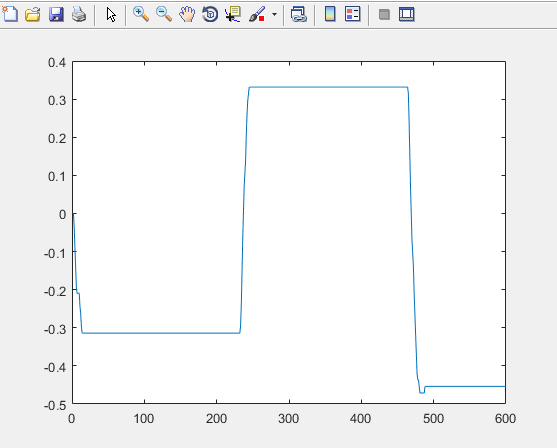
\includegraphics[width = 300pt]{figur/system_respons}
	\caption{System Respons}
	\label{fig:system_respons}
\end{figure}


Overføringsfunktionen bliver genereret ud fra funktionen \textit{tfest()}, som estimerer en overføring ud fra inputtet vs outputtet \textit{beta}. Hertil får vi overføringsfunktionen:

\begin{equation}
Tf(s) = \frac{5.029}{s^2 + 39.28 s + 717.9}
\end{equation}

\subsubsection{Pol placeringskontrol}
For at opfylde vores krav til dynamikken, forsøges der at placeres dominerede poler i systemet. Først findes damping ratio'en ($ \zeta $) ud fra valget om overshoot (OS) på følgende måde: 

\begin{equation}
\zeta = \frac{-\ln(OS/100)}{\sqrt{\pi^2+\ln^2(OS/100)}}
\end{equation} 

Dernæst findes båndbredden wn ud fra $ \zeta $ og valget om settling time (Ts) på følgede måde:

\begin{equation}
wn = \frac{4}{\zeta*Ts}
\end{equation} 

Til sidst kan den ønskede karakteristiske ligning (Gs) findes og ved:
\begin{equation}
G(s) = \frac{wn^2}{s^2+2*\zeta*wn*s+wn^2}
\end{equation}

Ud fra G(s) findes isoleres polerne, som skal bruges til at opfylde kravene om settling time (Ts) og overshoot (OS). For vores krav ligger polerne  derfor i -4\textpm\ 4.08i. For at fjerne steady state error tilføjes en ekstra pol i 5-10 gange real delen af de dominerende poler. Denne ekstra pol på reel aksen fungere som integrator i kontrolloopet, som korrigerer steady state error'en, men den øger også ordenen af systemet.


\subsubsection{State space model}

I dette projekt bliver systemet controller del repræsenteret på controller state space form, dette gøres for at kunne ændre på state vectorerne, som ændres vha. gainblokke (K), som bliver tilføjet til systemet. For at transformere transferfunktionen til en state space model, laves en state space tranformation i matlab. State space formlen giver følgende state space repræsentation

\begin{enumerate}
	
	\item
	$
	A = 
	\begin{bmatrix}
	
	-39.2765 & -717.8563 \\
	1.0000     &    0
	\end{bmatrix}
	$
	\item
	$
	B = 
	\begin{bmatrix}
	
	1\\
	0
	\end{bmatrix}
	$    
	
	\item 
	$
	C = 
	\begin{bmatrix}
	
	0  &  5.0293
	\end{bmatrix}
	$    
	\item
	$
	D = 
	\begin{bmatrix}
	
	0  
	\end{bmatrix}
	$  
\end{enumerate}      
Som vist tidligere, er der fundet nogle poler, som ønskes realiseret. Derfor indsættes en K matrix, som skal placeres, i tilbagekoblingen for at opnå de ønskede poler i close-loopet, dette ses nedenunder. 

\begin{lstlisting}[frame=single]
K = place(A,B,poles);
AA = A-B*(K);
sys=ss(AA,B,C,D);
\end{lstlisting}

Herved vises closed loop repræsentationen, for controller design, ift. kravene på overshoot og settling time.\\


HEREFTER KAN VI TILFØJE EN Ke, som regulerer på STEADY STATE ERROR (MANGLER KODE HERFRA). 



\subsection{Observer design}
Da systemet i praksis foregår på en motorblok, kan vi ikke hente de states matrixen, da x1 og x2 er en del  af systemet, ift ligningen for state space controller repræsentationen: 
\begin{gather}
\dot{x}=Ax+Bu \\
y=Cx
\end{gather}
Derfor indsættes yderligere en blok i systemet, for at kunne observere ind og output, og på baggrund af dem, og de beregnede state matrixes, beregnes en estimeret xhat, som skal bruges til tilbagekoblingen, som erstatning for states matrixen \\
Observer formlen hedder:


\begin{gather}
\dot{\hat{x}}=A\hat{x}+Bu+L(y-\hat{y}) \\
\hat{y}=C\hat{x}
\end{gather}

Vha af mellemregninger, får vi formlen: 
\begin{gather}
\dot{\hat{x}}=(A+BK-LC)\hat{x}+Ly \\
u=K\hat{x}
\end{gather}

Som er den formlen vi bruger til at lave vores observer.\\

Til observer tilføres en ny konstant L, som er udregnet til at styre observerens hastighed, så den er hurtigere end controlleren. L er beregnet ud fra formlen:
\begin{lstlisting}[frame=single]
L=place(A', C', poles)'
\end{lstlisting}

som er fundet her HENVISNING!!!

\subsection{Diskret controller design}
For at kunne implementere systemet på en microcontroller - som på LEGO EV3, kan systemet med fordel transformeres til en diskret state space model. Dette kommer af at reguleringen skal foregå på et digitalt system, som sampler med en bestemt frekvens. Både overføringsfunktionen og state space repræsentationen bliver transformeret til diskrete værdier, det samme gøres ved vores poler, hvormed K værdierne ændres til de passende værdier. Alt dette gøres igennem matlab, hvor funktionen c2d bliver brugt.




\pagebreak
\section{Simulation}
\subsection{Kontinuer controller}
For at teste den kontinuere controller's respons modelleres systemet ud fra state space repræsentationen og de fundne K-værdier til følgende blokdiagram \autoref{fig:Simulink_blokdiagram_1}, uden brug af observer i første omgang. 

\begin{figure}[H]
	\centering
	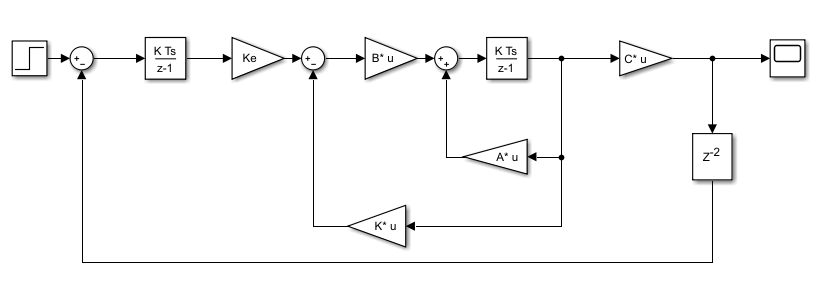
\includegraphics[width = 1\textwidth]{figur/Simulink_blokdiagram_1}
	\caption{Blok diagram for den kontinuere controller uden observer}
	\label{fig:Simulink_blokdiagram_1}
\end{figure}

State matricen hentes direkte fra modellen ligesom i Matlab. Delay blokken med 2 unit delay skyldes, at gerne vi simulere at gyroskopet på udgangen bruger 1 delay på at sample og 1 delay på at integrere den samplede vinkelhastighed til en vinkel. Ved at sende et step med amplituden 30 ind som reference signal forventer vi derfor, at kunne måle en værdi på 30 på outputtet efter cirka halvt sekund efter steppet. Dette kan ses i scopet i \autoref{fig:Simulink_scope_1}.

\begin{figure}[H]
	\centering
	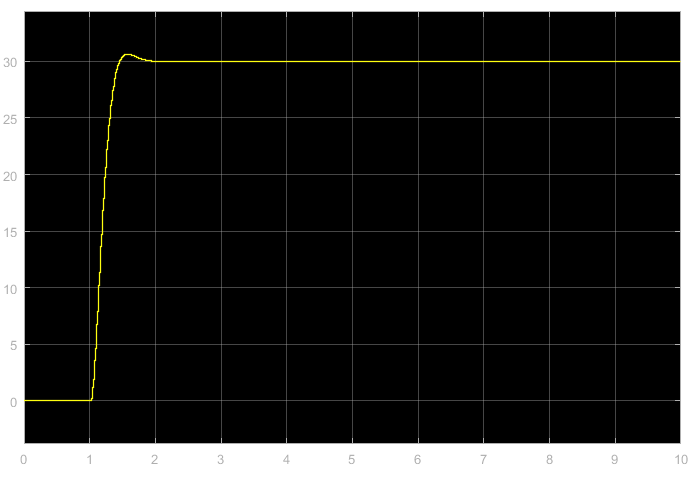
\includegraphics[width = 0.75\textwidth]{figur/Simulink_scope_1}
	\caption{Step respons (Amplitude = 30) for den kontinuere controller uden observer}
	\label{fig:Simulink_scope_1}
\end{figure}

Resultatet i \autoref{fig:Simulink_scope_1} passer med forventningerne med settling time og ingen steady state error. Dog ses der et lille overshoot på cirka 1.5\%, hvilket tyder på at systemet er blevet lidt mindre stabilt pga delay blokken med 2 unit delay. Dette har dog minimal betydning, da kravet om max 5\% overhoot stadig overholdes.

Men som nævnt tidligere kan man ikke hente state matricen direkte ud fra systemet, så derfor tilføjes en observer til blokdiagrammet i \autoref{fig:Simulink_blokdiagram_1} så state matrixen kan hentes fra outputtet i stedet. Dette kan ses herunder i \autoref{fig:Simulink_blokdiagram_2}.

\begin{figure}[H]
	\centering
	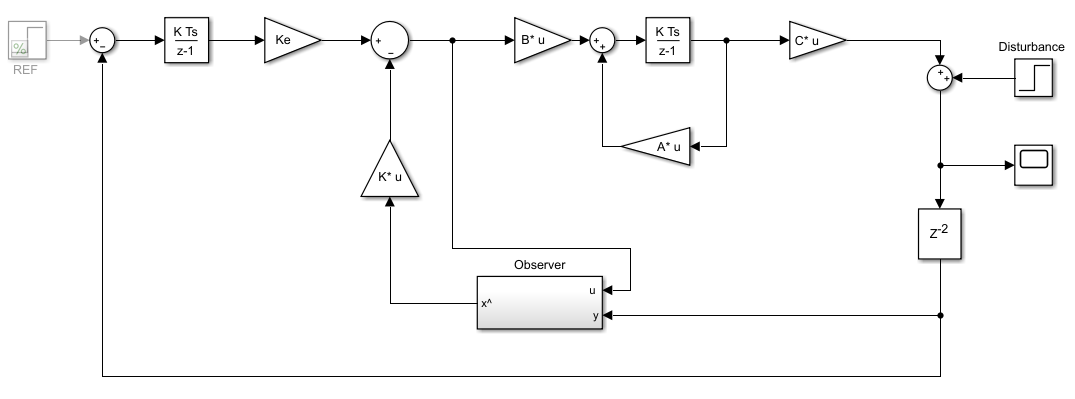
\includegraphics[width = 1\textwidth]{figur/Simulink_blokdiagram_2}
	\caption{Blok diagram for den kontinuere controller med observer}
	\label{fig:Simulink_blokdiagram_2}
\end{figure}
I \autoref{fig:Simulink_blokdiagram_2} ses det at observeren har outputtet fra gyroskoppet som input sammen med inputtet til motorblokken (state space repræsentation) og spytter states matricen ud, som føres tilbage med forstærkningensmatricen K . Observeren er implementeret ud fra det tidligere design og kan ses i \autoref{fig:Simulink_observer_continues}. Ved at sende et step med amplituden 30 ind som forstyrrelse signal på outputtet (forstyrrelse fra overfladens hælding) forventer vi derfor, at kunne måle en værdi på 0 på outputtet efter cirka halvt sekund efter steppet, hvis referencesignalet sættes til 0. Dette kan ses i scopet i \autoref{fig:Simulink_scope_2}.
 
\begin{figure}[H]
	\centering
	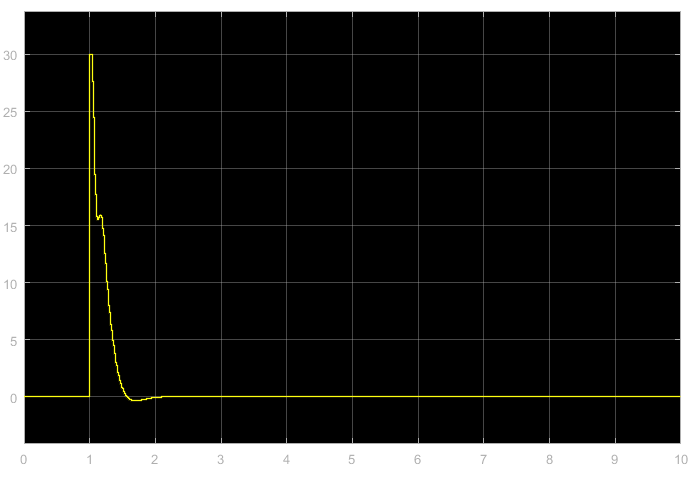
\includegraphics[width = 0.75\textwidth]{figur/Simulink_scope_2}
	\caption{Step respons for den kontinuere controller med observer påsat forstyrrelse på outputtet (Amplitude = 30)}
	\label{fig:Simulink_scope_2}
\end{figure}

Resultatet i \autoref{fig:Simulink_scope_2} passer med forventningerne og viser at systemet regulere tilbage til vandret efter cirka et halvt sekund, hvis det bliver udsat for en forstyrrelse. Dog ses det at, reguleringen ikke sker helt jævnt, hvilket formentlig skyldes at observeren påvirker systemet med sine poler og ikke gætter 100\% rigtig på state matricen, hvormed resultatet påvirkes. Dette er dog acceptabelt, idet systemet stadig finder tilbage på plads uden alt for meget oscillation. 

\subsection{Diskret controller}
For at teste den ufuldstændige diskrete controller's respons modelleres systemet ud fra state space repræsentationen og de fundne Kd-værdier til følgende blokdiagram \autoref{fig:Simulink_blokdiagram_3}, uden brug af observer i første omgang. 

\begin{figure}[H]
	\centering
	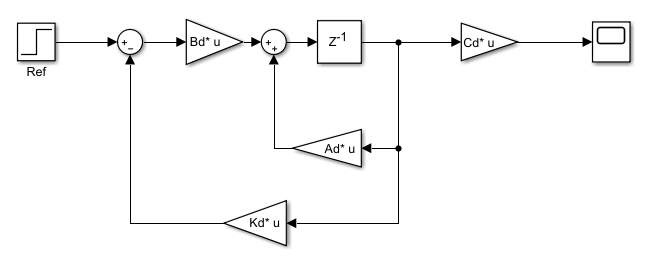
\includegraphics[width = 0.80\textwidth]{figur/Simulink_blokdiagram_3}
	\caption{Blok diagram for den diskrete controller uden observer og uden korrektion for steady state error}
	\label{fig:Simulink_blokdiagram_3}
\end{figure}

State matricen hentes direkte fra modellen ligesom i Matlab. Det er værd at bemærke, at hvor der før i den kontinuere state space model var et integrationsblok er denne ny byttet ud med en unit delay blok for at realisere den samplede state matrix. Ved at sende et step med amplituden 30 ind som reference signal forventer vi, at systemet falder til efter cirka halvt sekund efter steppet og ikke har noget betydeligt overshoot. Dette kan ses i scopet i \autoref{fig:Simulink_scope_3}.

\begin{figure}[H]
	\centering
	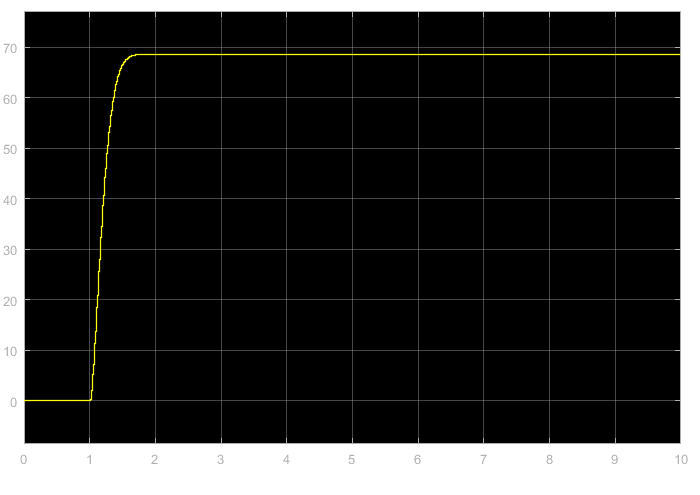
\includegraphics[width = 0.75\textwidth]{figur/Simulink_scope_3}
	\caption{Step respons (Amplitude = 30) for diskrete controller uden observer og uden korrektion for steady state error}
	\label{fig:Simulink_scope_3}
\end{figure}

Resultatet i \autoref{fig:Simulink_scope_1} passer med forventningerne med settling time og overshoot. Den stationære værdi er for høj, hvilket skyldes at denne controller ikke har nogen korrektion for steady state error med et integrationsled i loopet ligesom den kontinuere controller. Igen kan man ikke i praksis hente state matricen direkte ud fra systemet som her, så derfor tilføjes en observer til blokdiagrammet i \autoref{fig:Simulink_blokdiagram_3}, så state matrixen kan hentes fra outputtet i stedet. Dette kan ses herunder i \autoref{fig:Simulink_blokdiagram_4}.

\begin{figure}[H]
	\centering
	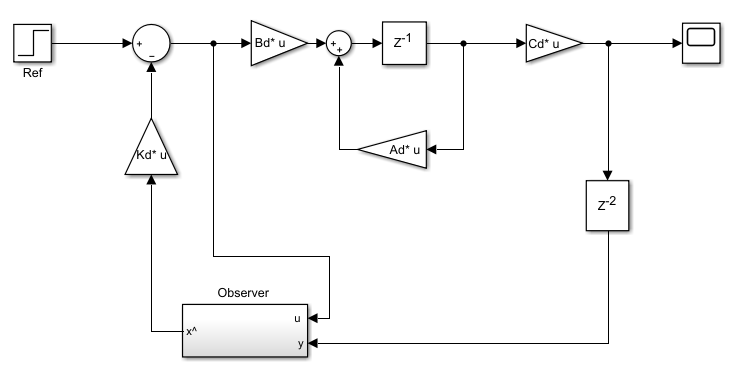
\includegraphics[width = 0.8\textwidth]{figur/Simulink_blokdiagram_4}
	\caption{Blok diagram for den diskrete controller med observer og uden korrektion for steady state error}
	\label{fig:Simulink_blokdiagram_4}
\end{figure}

I \autoref{fig:Simulink_blokdiagram_4} ses det, at observeren har outputtet fra gyroskoppet som input sammen med inputtet til motorblokken (state space repræsentation) og spytter states matricen ud, som føres tilbage med forstærkningensmatricen Kd. Observeren er implementeret ud fra det tidligere design og kan ses i \autoref{fig:Simulink_observer_diskret}. Ved igen at sende et step med amplituden 30 ind som reference signal, forventer vi at systemet falder til efter cirka halvt sekund efter steppet og ikke har noget betydeligt overshoot, præcis ligesom før uden observer. Dette kan ses i scopet i \autoref{fig:Simulink_scope_4}.

\begin{figure}[H]
	\centering
	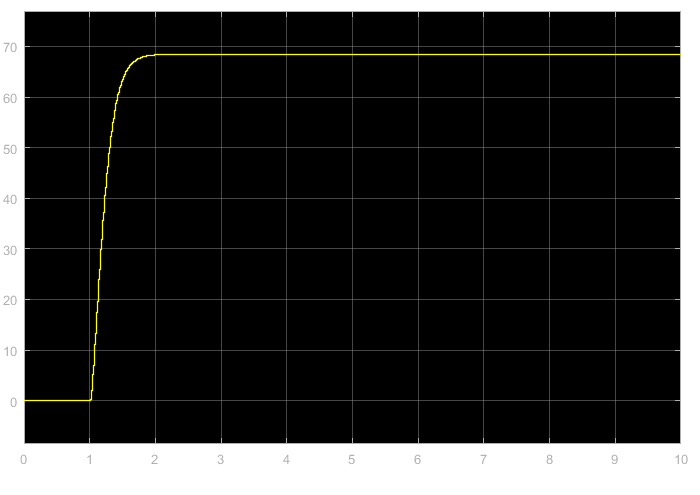
\includegraphics[width = 0.75\textwidth]{figur/Simulink_scope_4}
	\caption{Step respons (Amplitude = 30) for diskrete controller med observer og uden korrektion for steady state error}
	\label{fig:Simulink_scope_4}
\end{figure}

Resultatet i \autoref{fig:Simulink_scope_4} viser det samme som i \autoref{fig:Simulink_scope_3}, hvormed det kan konkluderes at observeren virker som forventet. Den eneste forskel er, at systemet virker en anelse langsommere, formentlig fordi observeren ikke gætter 100\% rigtig på state matricen, hvormed resultatet påvirkes.
 






\pagebreak
\section{Test på LEGO bil}


\pagebreak
\section{Adaptiv}

Gennem Design sektionen, kommer vi ikke ind på den adaptive del af projektet. Dette skyldes grundet tidsmangel, at gruppen ikke nåede at implementere et adaptiv regulerings feedback. I dette afsnit, vil der forklares om adaptiv controller, og hvordan det burde være implementeret til projektet. 

Problemene med et normalt kontrolsystem er, at dele af systemet kan være ukendt eller have ukendte parametre. Systemets parametre kan ofte varierer med tiden (slid på dæk, mindre vægt osv.), og systemet kan blive påvirket af ukendte forstyrrelser (støj, vind, varme), som ændre systemet karakteristik. Derfor indfører man ofte en adaptiv controller til at tilpasse sig ændringerne og til at ændre systemets adfærd til at overholde nye omstændigheder.
Følgende to regulatorer er eksempler på adaptive regulatorer, som kan løse overstående problemer.  


\subsection{MRAC regulator}
Model Reference Adaptive Control (MRAC) er en adaptiv regulator model, som bygger på en reference model af systemet.
MRAC designes normalt til at oprette en closed-loop controller med opdaterende parametre til at ændre systemets respons som ønsket. I modellen sammenlignes udgangen af systemet med et ønsket svar fra en referencemodel, og opdateringen af kontrol parametrene er baseret på denne fejl. Formålet med disse parametre er at matche de ønskede værdier, således at systemet output matcher referencemodellens output \cite{adaptive}.
Herunder vises hvordan et klassisk MRAC system ser ud:


\begin{figure}[H]
	\centering
	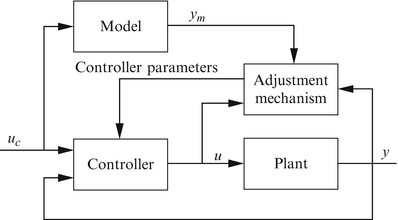
\includegraphics[width = 300pt]{figur/MRAC}
	\caption{Klassisk MRAC system}
	\label{fig:MRAC}
\end{figure}

For at bestemme den adjustment mechanism, som skal bringe fejlen mellem systemets output og referencemodellens output bruger man ofte den såkaldte MIT rule. MIT rule er en måde at beregne de adjustment mechanism, som vist på \autoref{fig:MRAC}, som skal til for at systemet opfører sig adaptiv. MIT-reglen kan betragtes som en gradient løsning for at minimere den kvadratiske fejl $e^{2}$. For at sikre stabilitet, kan den modificerede MIT rule benyttes. Dette gøres, hvis reference inputtet har store udsving, som kan gøre systemet ustabil. \\


\subsection{MIAC}
Til dette projekt, skulle der have været en adaptiv regulering, og derigennem var valget faldet på at bruge Model Identification Adaptive Control (MIAC). Ideen med et MIAC system er regulatoren hele tiden står og identificere processen, som kører ved hjælp af en estimator. Herefter gendesigner regulatoren selve controllerens parametere ud fra den fundne system model og kravene til responsen for systemet. Dette gør, at hvis systemets parametre har ændret sig i forhold til startparametrene, så tuner regulatoren selv centrolleren ind til de nye system parametre. Derfor kaldes denne type controller også ofte Self-tuning-regulator \cite{adaptive}. En anden fordel ved systemet er, at hvis det oprindelige controller design ikke passer helt med den reelle process, så tuner regulatoren også langsomt det delvist forkerte controller design ind til den ønskede respons. Herunder vises hvordan et klassisk MIAC system ser ud:

\begin{figure}[H]
	\centering
	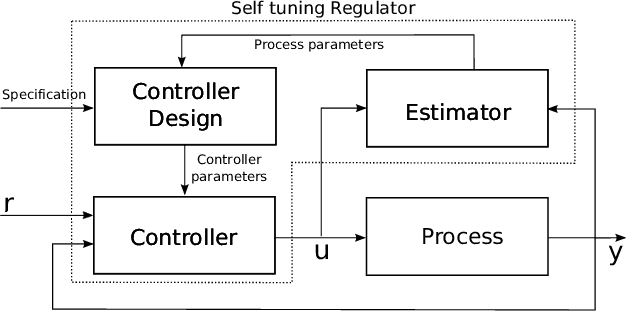
\includegraphics[width = 300pt]{figur/MIAC}
	\caption{Klassisk MIAC system}
	\label{fig:MIAC}
\end{figure}

\subsubsection{RLS}
Til MIAC skal der benyttes en estimation mekanisme, og derigennem blev der valgt at bruge Recursive least squares (RLS) algoritmen, da vi havde kendskab til denne metode gennem undervisningen, og fordi den er nem at tilgå. Her skulle systemets estimation mekanisme laves ud fra online RLS, da systemet skal kunne køre i reel tid og derfor ikke har et hele udgangssignalet for processen. 

RLS algoritmen er en adaptiv filteralgoritme, der recursivt finder koefficienterne(estimation), der minimerer en vægtet lineær least squared kostprisfunktion i forbindelse med indgangssignalerne versus udgangssignalerne. Til realiseringen af det adaptive system, var planen at indsætte RLS algoritmen i system estimator blokken, som ses på \autoref{fig:MIAC}. Hertil skulle der laves en regulerings blok, som regulerede på K værdierne i forhold til de valgte specifikationer som på \autoref{fig:Blokdiagram}.
RLS algoritmen, ville levere en estimation af systemet Thetahat. RLS algoritmen kan ses i \autoref{fig:RLS_formel} 


 \begin{figure}[H]
	\centering
	
\includegraphics[width = 300pt]{figur/RLS_formel}
	\caption{Formel for theta fra RLS online blokken}
	\label{fig:RLS_formel}
\end{figure}
Hvor Phi er de kendte værdier, in- og output sat sammen i en samlet vektor,  mens Thetahat er model parmenterne for systemet (estimation) sat sammen i en samlet vektor 

\subsubsection{Glemselsfaktor og Kalman filter}  
Det endelige RLS system kan forbedres med flere faktorer, her vil vi kort forklare om de to tilføjelser, som er blevet præsenteret til undervisningen, og som RLS algoritmen kan udvides med.

\textbf{Glemselsfaktor}
Glemselsfaktoren gør det, at modellen kigger mere på de forrige samples end de tidlige, og derfor ikke kigger jævnt  på hele signalet. Dette gør systemet hurtigere overfor ændringer, da den nye sampling med ændringen vejere tungere end tidligere samples. Dette fjerne modelstøjen fra estimationen, hvis processens karatestik er tidsafhængig. 

\textbf{Kalman filter}
RLS antager, at der ikke er noget målestøj, og at det vi måler præcis er input og output. Kalman filteret er godt i de situationer, hvor der tilføres støj til systemet, som reelt set altid vil være i en virkelig implementering. Her er Kalman filteret ikke så modtagelig overfor støj, og derved bedre til at estimere de korrekte værdier end standard RLS.



%\pagebreak
%\section{Diskussion}



\pagebreak
\section{Konklusion}
Det kan konkluderes, at kan lade sig gøre at udnytte den dipole egenskab i en planar ribbon tweeter, vha. bagside-reflektorer til at bidrage med mere diskant til siderne, og dermed skabe en mere rumlig og levende lyd.
I projektet opstod de bedste resultater ved at bruge en reflektor med lige sider (ret trekant). 
Dette gav den mest klare og afbalancerede mængde diskant i $90 ^{\circ}$ fra højtaleraksen.
Det kan også konkluderes, at højtalerdesignet ikke er fejlfrit, men stadig har opnået de væsentligste designegenskaber, som blev valgt til formålet med dette projekt. 


\pagebreak
\bibliography{References}{}
\bibliographystyle{plain}

\end{document}